\chapter{Introdução}\label{sec:introducao}
A violência de gênero representa uma das mais graves violações dos direitos humanos na sociedade contemporânea, constituindo-se como uma problemática estrutural que transcende fronteiras geográficas, classes sociais e contextos culturais. No Brasil, os dados estatísticos recentes revelam um cenário alarmante que demanda intervenções tecnológicas urgentes e inovadoras para a proteção de pessoas em situação de vulnerabilidade.

Segundo dados oficiais compilados pelo Sistema Nacional de Informações de Segurança Pública (Sinesp), o país registrou 1.450 casos de feminicídio em 2024, representando um aumento em relação ao ano anterior\cite{sinesp2024feminicidio}. Esta estatística traduz-se em uma realidade devastadora: a cada 17 horas, ao menos uma mulher foi vítima de feminicídio no território nacional. Nos casos de feminicídio, os dados revelam características particularmente preocupantes: 80\% das mulheres assassinadas foram mortas por companheiros ou ex-companheiros, 64\% dentro da própria residência, e 64\% eram mulheres negras.

O panorama da violência sexual apresenta dimensões igualmente alarmantes, com o Brasil registrando mais de 87 mil casos de estupro em 2024. A residência configura-se como o local de maior risco para as mulheres, sendo onde ocorrem 71,6\% das notificações de violência doméstica, sexual e outras formas de violência contra mulheres, com 76,6\% dos agressores sendo do sexo masculino.

Para além da violência direcionada especificamente contra mulheres, a população LGBTQIAPN+ enfrenta índices crescentes de violência motivada por discriminação de gênero e orientação sexual. O Brasil registrou 291 mortes violentas de pessoas LGBTQIAPN+ em 2024, representando um aumento de 13,2\% em relação ao ano anterior, segundo levantamento do Observatório do Grupo Gay da Bahia\cite{grupogay2024bahia}. Dados do Observatório Nacional dos Direitos Humanos indicam que 11.120 pessoas LGBTQIA+ foram vítimas de algum tipo de agressão em função da orientação sexual ou identidade de gênero em 2022, com pessoas transexuais e travestis correspondendo à maioria dos casos (38,5\%). O Atlas da Violência demonstra que nos últimos 10 anos, os casos registrados de violência contra a população LGBTQIAPN+ aumentaram em 1227\%\cite{observaDH2024}.

Particularmente preocupante é a situação das pessoas trans, onde a média de idade das travestis e transexuais assassinadas em 2024 é de 24,64 anos \cite{antra2024dossiê}, evidenciando que a maioria dessas pessoas, predominantemente profissionais do sexo, perde a vida antes mesmo de atingir os 35 anos.

Diante desta realidade, evidencia-se a necessidade urgente de desenvolvimento de soluções tecnológicas que possam oferecer ferramentas de proteção e socorro para pessoas em situação de vulnerabilidade e risco iminente. A tecnologia mobile, com sua penetração massiva na sociedade brasileira e capacidades de geolocalização em tempo real, apresenta-se como uma alternativa viável para a criação de mecanismos de resposta rápida em situações de emergência.

Neste contexto, o presente trabalho tem como objetivo o desenvolvimento de uma aplicação móvel denominada "SheSafe", concebida como uma ferramenta tecnológica de proteção e socorro direcionada prioritariamente a mulheres em situação de violência doméstica e de gênero, mas extensível a todas as pessoas que se encontrem em situações de vulnerabilidade e risco, incluindo a população LGBTQIAPN+. A aplicação visa implementar funcionalidades de envio automatizado de pedidos de socorro com coordenadas de geolocalização precisas, permitindo resposta rápida de redes de apoio e órgãos competentes.

A relevância social desta proposta fundamenta-se na crescente demanda por ferramentas que possam atuar como mecanismos de proteção complementares às políticas públicas existentes, oferecendo às vítimas uma alternativa discreta e eficiente para solicitação de auxílio em momentos críticos. A integração de tecnologias de geolocalização com sistemas de comunicação instantânea representa uma abordagem inovadora no enfrentamento à violência de gênero, podendo contribuir significativamente para a redução dos índices de violência e para a preservação de vidas.

Do ponto de vista técnico, o desenvolvimento da aplicação SheSafe envolve a integração de tecnologias contemporâneas de desenvolvimento mobile, incluindo a plataforma Android, o framework Firebase para gerenciamento de dados e autenticação, e APIs de geolocalização para determinação precisa de coordenadas. Esta solução tecnológica representa uma contribuição concreta para o enfrentamento de uma problemática social de extrema relevância, alinhando inovação tecnológica com responsabilidade social.

\section{Objetivo do Projeto}
Desenvolver uma aplicação móvel denominada "SheSafe" para envio automatizado de pedidos de socorro com coordenadas de geolocalização em tempo real, direcionada prioritariamente a mulheres vítimas de violência doméstica e de gênero, mas extensível a todas as pessoas em situação de vulnerabilidade, incluindo a população LGBTQIAPN+.

%O escopo do projeto tem como base oferecer uma aplicação simples, intuitiva e de fácil acesso ao nosso público-alvo para que estes sejam capazes de enviar um pedido de ajuda, para pessoas de sua confiança, em momentos que estiverem passando por uma situação de risco, agressão ou até mesmo violência. Estes pedidos de ajuda informarão a essas pessoas de confiança, na aplicação denominadas de “contatos seguros”, a localização atual do usuário juntamente com uma mensagem predefinida por ele.

%\section{Público-alvo}
%SheSafe tem como público-alvo pessoas do sexo feminino que desejam ter uma forma de comunicar a pessoas de sua confiança algum potencial risco; seja ele violência, agressão, insegurança na rua, perseguição por algum individuo ou outro risco qualquer, que estiver passando em tempo real

\section{Mapa de empatia inicial}
\begin{figure}[htbp]
  \begin{center}
  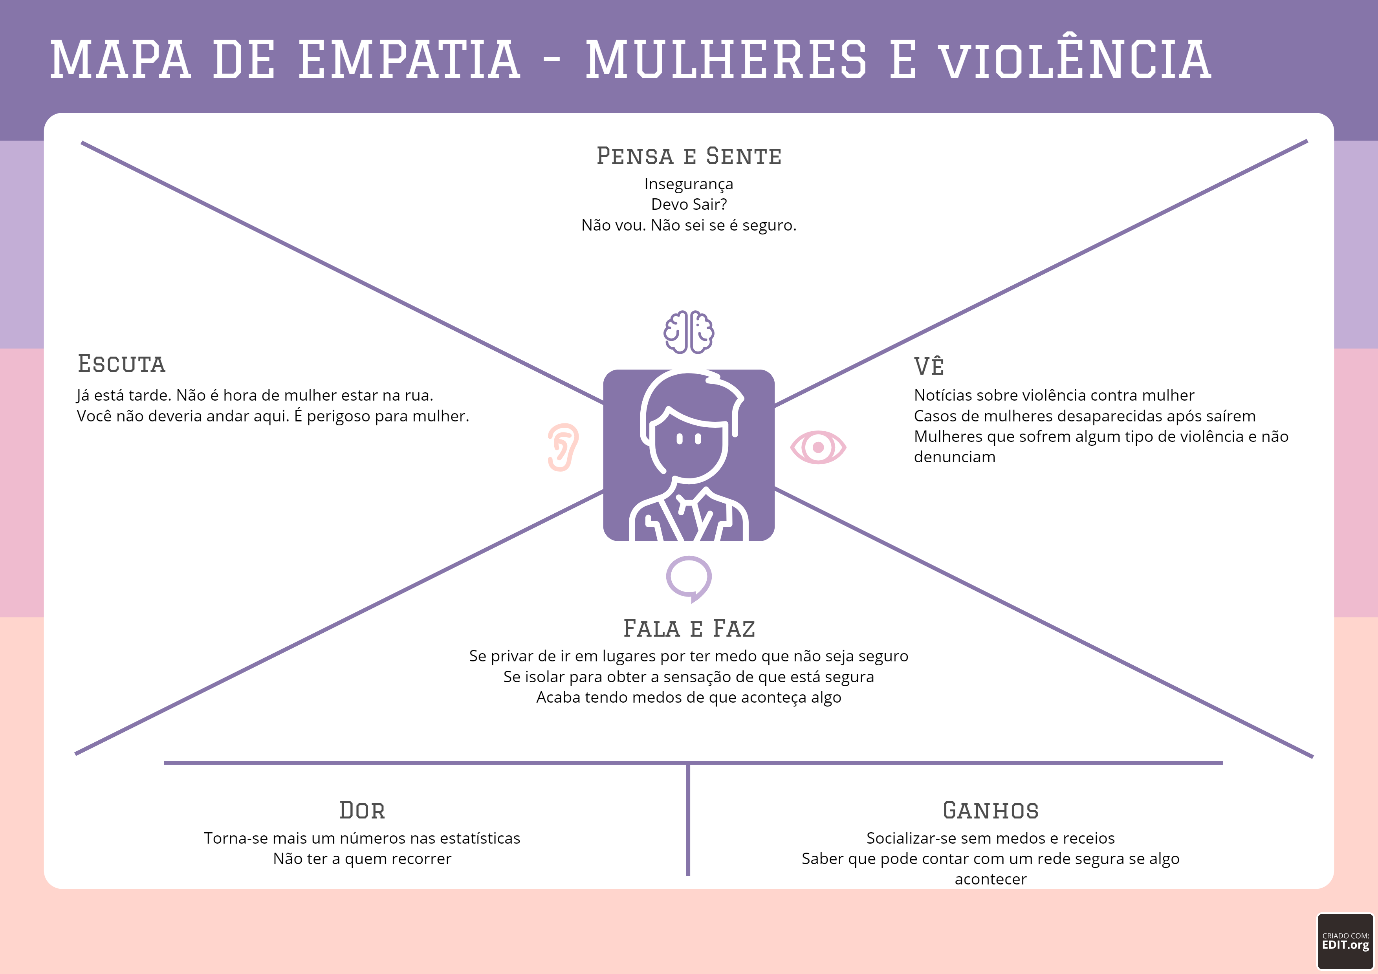
\includegraphics[width=.9\linewidth]{images/mapa-empatia-inicial.png}\\
  \end{center}
  \caption[Mapa de empatia inicial]{Mapa de empatia inicial sobre sentimento das mulheres sobre violência}
  \label{fig:mapa-empatia-inicial}
  \legend{Fonte: Próprio Autor}
\end{figure}
\pagebreak

\section{Ambiente de uso}
O SheSafe poderá ser utilizado em qualquer ambiente desde que se tenha um plano de internet ativo para que os pedidos de ajuda possam ser enviados corretamente para a lista de contatos seguros. Uma outra restrição quanto ao uso é que os usuários devem possuir um smartphone com sistema operacional Android ou iOS para que possam instalar o aplicativo.

\section{Restrições de Uso/Circunstâncias}
Não há restrições quanto ao uso do SheSafe. Caso o usuário sinta-se em situação de risco ele poderá acionar o aplicativo e enviar seu pedido de ajuda, desde que já tenha cadastrado sua lista de contatos seguros.

\section{Diferencial}
Dado que muito dos casos de agressão acontecem com mulheres em situação de risco e muitas das vezes elas são privadas de acesso a formas de comunicação mais tecnológicas, o intuito é ter uma aplicação onde as mulheres possam reportar crimes de forma simples, prática e disponível para todos os públicos. O principal diferencial está em não restringir o acesso a aplicação para nosso público-alvo e ter a opção de envio da localização no momento do acontecimento.

\section{Funcionalidades mínimas para garantir a relevância do aplicativo}
As funcionalidades mínimas elencadas para que o projeto tenha relevância são:
\begin{alineas}
  \item Login: Para criação de usuário
  \item Pedido de socorro: Botão para acionar pedido de socorro
  \item Lista Segura: Gerenciamento de contatos seguros
  \item Perfil: Página para alteração da mensagem de socorro

\end{alineas}
